\documentclass[twocolumn,showpacs,preprintnumbers,amsmath,amssymb,pra,floatfix]{revtex4-2}

% Standard packages
\usepackage[T1]{fontenc}
\usepackage{graphicx}
\usepackage{booktabs}
\usepackage{hyperref}
\usepackage{siunitx}
\usepackage{algorithm}
\usepackage{algpseudocode}
\usepackage{bm}
\usepackage{dcolumn}
\usepackage{braket}
\usepackage[section]{placeins}


\graphicspath{{figures/}}

% Aggressive float placement parameters to avoid stuck floats in twocolumn
\renewcommand{\topfraction}{0.9}
\renewcommand{\bottomfraction}{0.9}
\renewcommand{\textfraction}{0.1}
\renewcommand{\floatpagefraction}{0.8}
\renewcommand{\dbltopfraction}{0.9}
\renewcommand{\dblfloatpagefraction}{0.8}
\setcounter{topnumber}{4}
\setcounter{bottomnumber}{4}
\setcounter{totalnumber}{8}
\setcounter{dbltopnumber}{4}

\hypersetup{
    colorlinks=true,
    linkcolor=blue,
    citecolor=blue,
    urlcolor=blue
}

\begin{document}

\preprint{arXiv:2511.12799v2}

\title{Numerical GRAPE optimization of single-qubit gates in a three-level transmon model:\\Leakage suppression and error budget analysis with hardware-representative parameters}

\author{Rylan Malarchick}
\affiliation{Department of Engineering Physics, Embry-Riddle Aeronautical University, Daytona Beach, FL 32114, USA}
\email{malarchr@erau.edu}

\date{\today}

\begin{abstract}
We present a systematic numerical comparison of Gaussian, derivative removal by adiabatic gate (DRAG), and gradient ascent pulse engineering (GRAPE) control pulses for single-qubit gates on a three-level transmon model with hardware-representative parameters from IQM's Garnet processor ($T_1 = \SI{37}{\micro\second}$, $T_2 = \SI{9.6}{\micro\second}$, $\alpha/2\pi = \SI{-200}{\mega\hertz}$). In the closed three-level system at a gate time of \SI{20}{\nano\second}, GRAPE achieves unit fidelity ($1 - F < 10^{-15}$) with negligible leakage ($P_2 < 10^{-16}$), compared to $F = 0.972$ for Gaussian pulses ($P_2 = 6.4 \times 10^{-4}$) and $F = 0.9995$ for DRAG ($P_2 = 1.2 \times 10^{-4}$). An error budget analysis using the Lindblad master equation shows that GRAPE's coherent error vanishes to machine precision, placing it at the decoherence floor ($1 - F = 7.2 \times 10^{-4}$), while Gaussian pulses are dominated by coherent error $39\times$ larger. Properly calibrated DRAG achieves coherent infidelity of only $4.9 \times 10^{-4}$, placing it close to the decoherence floor ($1 - F = 8.4 \times 10^{-4}$ with full decoherence) and within a factor of $1.2$ of GRAPE's open-system performance. A gate-time sweep from 10 to \SI{100}{\nano\second} reveals that both GRAPE and DRAG fidelities improve monotonically with gate time, while DRAG's leakage suppression improves exponentially---confirming the effectiveness of the analytical first-order correction when the DRAG parameter $\beta = -1/(2\alpha)$ is properly computed. Robustness analysis reveals that DRAG is \emph{more robust} than GRAPE to detuning errors (minimum fidelity 0.990 vs.\ 0.931 over $\pm\SI{5}{\mega\hertz}$), while GRAPE retains superior amplitude-error tolerance. All simulations and the open-source QubitPulseOpt framework are available at \url{https://github.com/rylanmalarchick/QubitPulseOpt}.
\end{abstract}

\pacs{03.67.Lx, 85.25.Cp, 03.65.Yz}

\maketitle

%==============================================================================
\section{Introduction}
\label{sec:introduction}
%==============================================================================

High-fidelity single-qubit gates are a prerequisite for fault-tolerant quantum computation~\cite{preskill2018quantum, knill2005quantum, arute2019quantum}. In superconducting transmon qubits~\cite{koch2007charge, krantz2019quantum, kjaergaard2020superconducting}, the weakly anharmonic energy spectrum creates a persistent tension: fast gates require strong driving fields that couple the computational subspace $\{\ket{0}, \ket{1}\}$ to higher transmon levels, introducing leakage errors that are not correctable by standard quantum error correction codes~\cite{aliferis2007fault, ghosh2013understanding}. This leakage-speed tradeoff is the central challenge for single-qubit gate optimization in transmon architectures~\cite{blais2021circuit}.

The derivative removal by adiabatic gate (DRAG) protocol~\cite{motzoi2009simple, gambetta2011analytic} provides a first-order analytical correction that adds a derivative component to the quadrature control channel, suppressing transitions to the $\ket{2}$ state. DRAG has been widely adopted in experimental practice and achieves high fidelities when properly calibrated~\cite{chen2016measuring, sheldon2016procedure}. However, DRAG is a perturbative correction valid to first order in $\Omega/\alpha$ (the ratio of Rabi frequency to anharmonicity) and does not account for higher-order leakage pathways or non-perturbative effects at short gate times.

Numerical optimal control methods~\cite{glaser2015training}, particularly the gradient ascent pulse engineering (GRAPE) algorithm~\cite{khaneja2005optimal}, can in principle discover pulse shapes that suppress leakage to arbitrary order by optimizing directly over the full multi-level Hilbert space. GRAPE has been successfully applied to superconducting qubit gates~\cite{lucero2010reduced, kelly2014optimal, werninghaus2021leakage, propson2022robust}, nitrogen-vacancy centers~\cite{dolde2014high}, and trapped ions~\cite{nebendahl2009optimal}. The key advantage of numerical optimization is its ability to exploit the full control landscape without perturbative approximations.

Despite the extensive literature on both DRAG and GRAPE, systematic comparisons under identical conditions with hardware-representative parameters remain surprisingly sparse. Many GRAPE demonstrations compare against uncalibrated baselines, while DRAG studies focus on two-level models where leakage is absent by construction. A rigorous comparison requires: (i) a multi-level transmon model that captures leakage physics, (ii) realistic device parameters from contemporary hardware, (iii) an error budget decomposing coherent and incoherent contributions, and (iv) robustness analysis against calibration imperfections.

In this paper, we address this gap through four systematic experiments using a three-level transmon model parameterized by calibration data representative of IQM's Garnet processor~\cite{iqm2024garnet}. We compare Gaussian, DRAG, and GRAPE pulses for the X gate across gate times from 10 to \SI{100}{\nano\second}, decompose the error budget into coherent, $T_1$, $T_2$, and control noise contributions using the Lindblad master equation~\cite{lindblad1976generators, breuer2002theory}, and analyze robustness to detuning and amplitude errors. Our results show that properly calibrated DRAG performs remarkably well---achieving closed-system fidelity $F = 0.9995$ at \SI{20}{\nano\second}---and that GRAPE's advantage lies primarily in eliminating \emph{all} coherent error to machine precision and in achieving superior performance at short gate times where perturbative corrections are insufficient.

The remainder of this paper is organized as follows. Section~\ref{sec:theory} presents the theoretical model. Section~\ref{sec:methods} describes the computational methods and pulse construction. Section~\ref{sec:results} presents results from all four experiments. Section~\ref{sec:discussion} discusses the findings in context. Section~\ref{sec:conclusion} concludes with future directions.

%==============================================================================
\section{Theoretical Model}
\label{sec:theory}
%==============================================================================

\subsection{Three-level transmon Hamiltonian}

We model the transmon as a weakly anharmonic oscillator truncated to three levels ($\ket{0}$, $\ket{1}$, $\ket{2}$). In the frame rotating at the qubit frequency $\omega_q$, the drift Hamiltonian is~\cite{koch2007charge}
\begin{equation}
H_d = \frac{\alpha}{2} \hat{n}(\hat{n} - \hat{I}),
\label{eq:drift}
\end{equation}
where $\alpha < 0$ is the anharmonicity and $\hat{n} = a^\dagger a$ is the number operator, with $a$ ($a^\dagger$) the bosonic annihilation (creation) operators truncated to the three-level subspace. In matrix form, $H_d = \text{diag}(0, 0, \alpha)$, so the $\ket{0} \leftrightarrow \ket{1}$ transition is resonant in the rotating frame and the $\ket{1} \leftrightarrow \ket{2}$ transition is detuned by $\alpha$.

The control Hamiltonian describes microwave driving through in-phase ($I$) and quadrature ($Q$) channels:
\begin{equation}
H_c(t) = \Omega_I(t) H_x + \Omega_Q(t) H_y,
\label{eq:control}
\end{equation}
where $\Omega_I(t)$ and $\Omega_Q(t)$ are the time-dependent control amplitudes (in rad/ns) and
\begin{align}
H_x &= \tfrac{1}{2}(a + a^\dagger), \label{eq:hx} \\
H_y &= \tfrac{1}{2}i(a^\dagger - a). \label{eq:hy}
\end{align}
The factor of $1/2$ follows the convention where $\Omega_I$ is the Rabi frequency. The total Hamiltonian is $H(t) = H_d + H_c(t)$.

For the two-level model used in validation experiments, we set $H_d = 0$ (resonant driving in the rotating frame) and replace $H_x, H_y$ with $\sigma_x/2, \sigma_y/2$.

\subsection{Pulse parameterization}

\subsubsection{Gaussian pulse}

The Gaussian pulse drives only the $I$-channel (Fig.~\ref{fig:pulses}a):
\begin{equation}
\Omega_I(t) = A \exp\left[-\frac{(t - T/2)^2}{2\sigma^2}\right], \quad \Omega_Q(t) = 0,
\label{eq:gaussian}
\end{equation}
where $T$ is the gate duration, $\sigma = T/(2n_\sigma)$ with $n_\sigma = 4$, and the amplitude $A$ is chosen to achieve a $\pi$-rotation:
\begin{equation}
A = \frac{\pi}{\sigma\sqrt{2\pi}}.
\label{eq:gaussian_amp}
\end{equation}

\subsubsection{DRAG pulse}

The DRAG protocol~\cite{motzoi2009simple} adds a derivative correction on the quadrature channel:
\begin{equation}
\Omega_Q(t) = \beta \frac{d\Omega_I}{dt},
\label{eq:drag}
\end{equation}
where the DRAG parameter is~\cite{motzoi2009simple, gambetta2011analytic}
\begin{equation}
\beta = -\frac{1}{2\alpha}
\label{eq:beta}
\end{equation}
with $\alpha$ the anharmonicity in angular frequency units (rad/ns). This expression arises from adiabatic elimination of the $\ket{2}$ state in the rotating frame, yielding a first-order correction that cancels the leading leakage term~\cite{motzoi2009simple}. Crucially, $\beta$ depends \emph{only} on the anharmonicity and is independent of the pulse amplitude and gate time.

For our parameters ($\alpha/2\pi = \SI{-200}{\mega\hertz}$, i.e., $\alpha = -1.257$ rad/ns), Eq.~\eqref{eq:beta} gives $\beta = 0.398$, an $O(1)$ quantity as expected from the perturbative derivation. Note that unit consistency is essential: if $\alpha$ is specified in MHz, it must be converted to rad/ns via $\alpha_\text{rad/ns} = 2\pi \times \alpha_\text{MHz} \times 10^{-3}$ before computing $\beta$.

\subsubsection{GRAPE pulse}

The GRAPE algorithm~\cite{khaneja2005optimal} represents the control pulse as piecewise-constant amplitudes $\{\Omega_I^{(k)}, \Omega_Q^{(k)}\}$ for $k = 1, \ldots, N$ time slices of duration $\delta t = T/N$. These $2N$ parameters are optimized to maximize the gate fidelity (Sec.~\ref{sec:fidelity}).


\begin{figure}[!htbp]
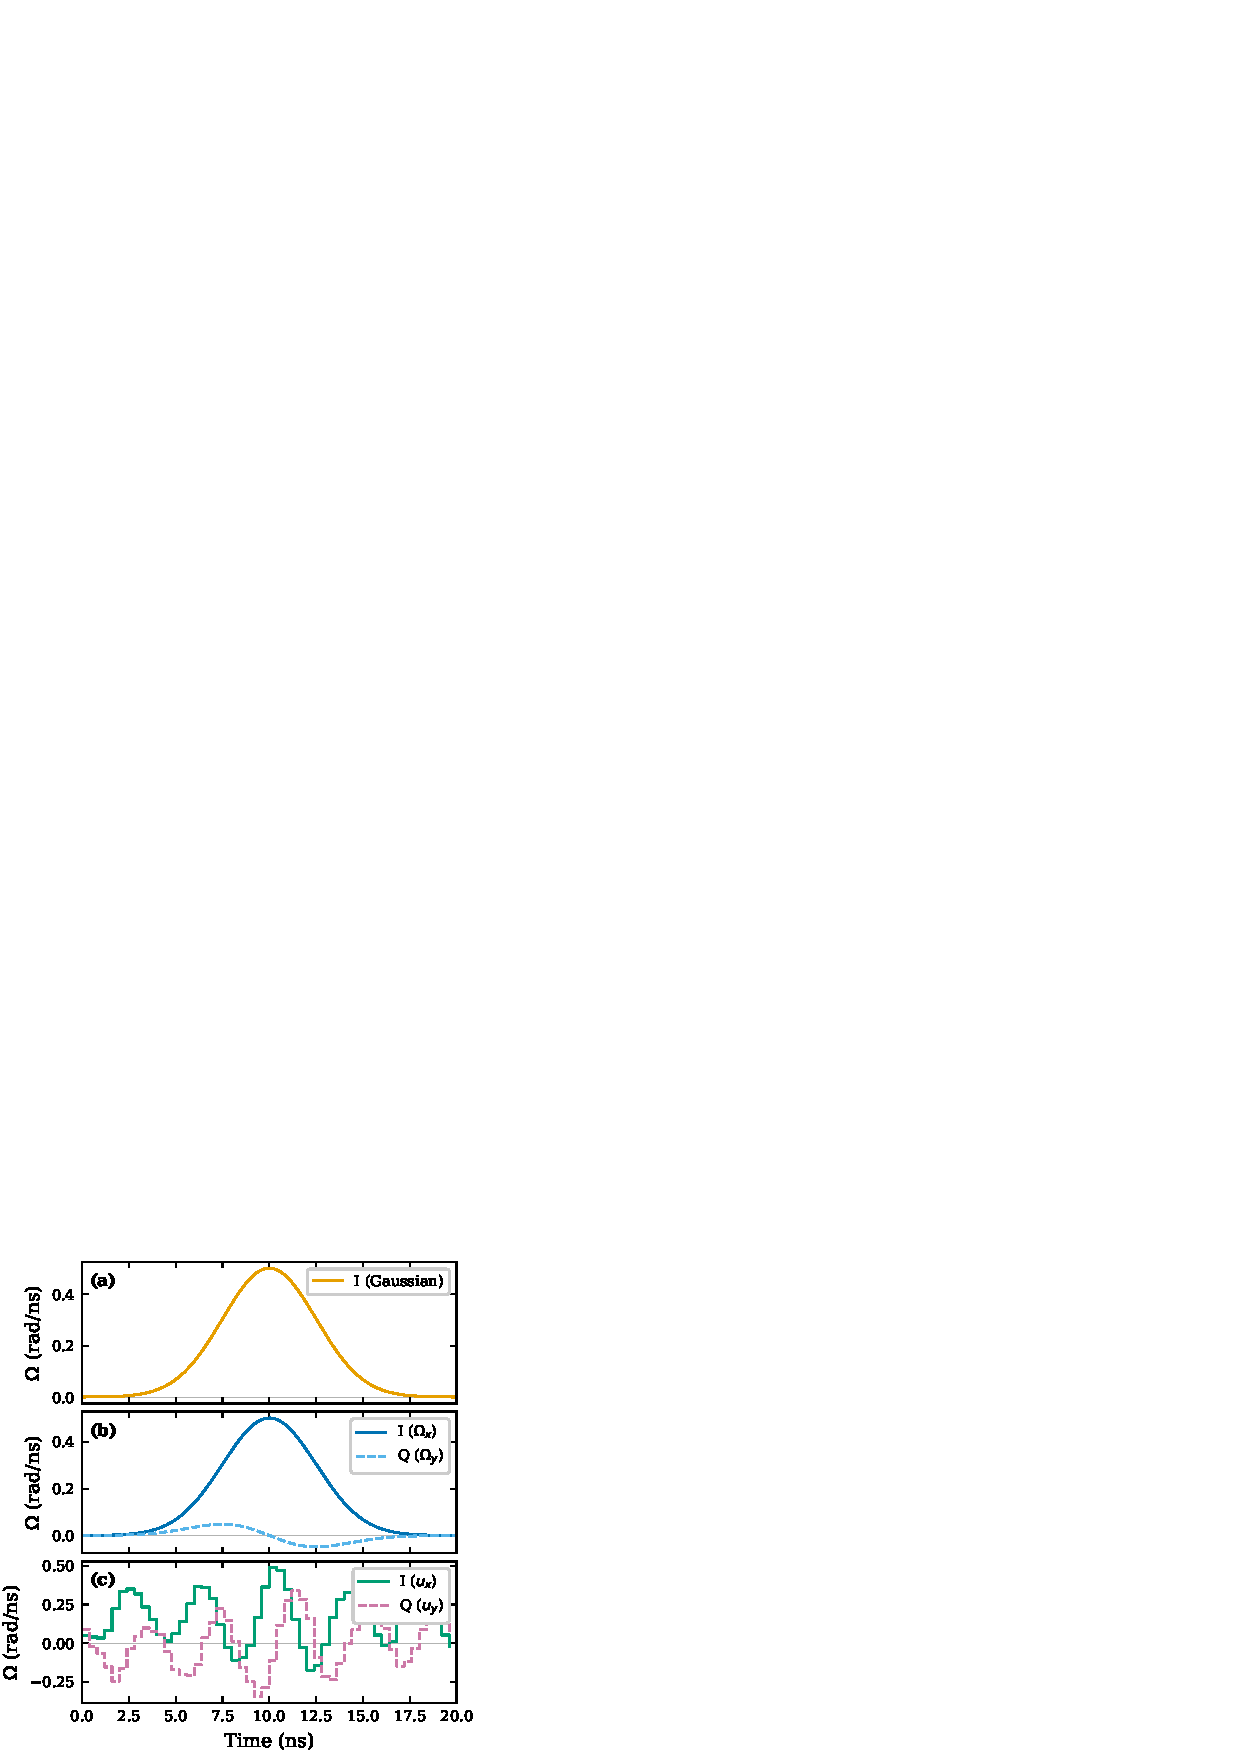
\includegraphics[width=\columnwidth]{fig1_pulse_shapes.pdf}
\caption{Control pulse waveforms for the X gate on a three-level transmon ($T = \SI{20}{\nano\second}$, $\alpha/2\pi = \SI{-200}{\mega\hertz}$). (a)~Gaussian pulse: in-phase ($I$) channel only. (b)~DRAG pulse: the $I$-channel carries the Gaussian envelope while the quadrature $Q$-channel applies the derivative correction $\Omega_Q = \beta\, d\Omega_I/dt$ with $\beta = 0.398$. (c)~GRAPE-optimized pulse: both $I$ and $Q$ channels are piecewise-constant with $N = 50$ time slices, showing the richer spectral content discovered by numerical optimization.}
\label{fig:pulses}
\end{figure}

\subsection{Gate fidelity}
\label{sec:fidelity}

For closed-system (unitary) evolution, we define the gate fidelity as
\begin{equation}
F = \frac{1}{d^2} \left|\text{Tr}(U_\text{target}^\dagger U_\text{final})\right|^2,
\label{eq:fidelity}
\end{equation}
where $U_\text{final}$ is the propagator resulting from the applied pulse, $U_\text{target}$ is the desired unitary, and $d$ is the dimension of the target subspace. For three-level simulations targeting a two-qubit gate (e.g., the X gate acting on $\{\ket{0}, \ket{1}\}$), $U_\text{target}$ is the $2 \times 2$ gate embedded as the upper-left block of a $3 \times 3$ unitary with identity action on $\ket{2}$, and $d = 2$. The fidelity is evaluated by projecting $U_\text{final}$ onto the computational subspace.

Leakage probability is defined as
\begin{equation}
P_2 = 1 - \sum_{j \in \{0,1\}} |\langle j | U_\text{final} | \psi_\text{init} \rangle|^2,
\label{eq:leakage}
\end{equation}
averaged over initial states $\ket{0}$ and $\ket{1}$.

\subsection{Open-system dynamics}
\label{sec:lindblad}

Decoherence is modeled by the Lindblad master equation~\cite{lindblad1976generators}:
\begin{equation}
\frac{d\rho}{dt} = -i[H(t), \rho] + \sum_k \left(L_k \rho L_k^\dagger - \frac{1}{2}\{L_k^\dagger L_k, \rho\}\right),
\label{eq:lindblad}
\end{equation}
with collapse operators for amplitude damping ($T_1$) and pure dephasing:
\begin{align}
L_1 &= \sqrt{\gamma_1}\, a, \quad \gamma_1 = 1/T_1, \label{eq:t1} \\
L_2 &= \sqrt{\gamma_\phi}\, \hat{n}, \quad \gamma_\phi = 1/T_2 - 1/(2T_1). \label{eq:t2}
\end{align}
For the three-level system, $a$ is the $3 \times 3$ annihilation operator and $\hat{n}$ is the number operator, naturally generalizing the two-level $\sigma_-$ and $\sigma_z/2$ collapse operators. The constraint $T_2 \leq 2T_1$ ensures $\gamma_\phi \geq 0$.

The process fidelity under open-system evolution is computed as
\begin{equation}
F_\text{proc} = \frac{1}{d} \sum_{j=0}^{d-1} \langle j | U_\text{target}^\dagger \rho_j(T) U_\text{target} | j \rangle,
\label{eq:process_fidelity}
\end{equation}
where $\rho_j(T)$ is the final density matrix when initializing in $\ket{j}$.

%==============================================================================
\section{Computational Methods}
\label{sec:methods}
%==============================================================================

\subsection{GRAPE optimization}

We implement the GRAPE algorithm following Khaneja \textit{et al.}~\cite{khaneja2005optimal}. The total propagator is constructed as
\begin{equation}
U_\text{final} = \prod_{k=N}^{1} U_k, \quad U_k = \exp\left(-i H_k \delta t\right),
\label{eq:propagator}
\end{equation}
where $H_k = H_d + \Omega_I^{(k)} H_x + \Omega_Q^{(k)} H_y$ is the Hamiltonian during the $k$-th time slice. The gradient of the fidelity with respect to the control amplitude $\Omega_c^{(k)}$ (for control channel $c \in \{I, Q\}$) is computed as~\cite{khaneja2005optimal, degroot2024grape}
\begin{equation}
\frac{\partial F}{\partial \Omega_c^{(k)}} = \frac{2}{d^2} \text{Re}\left[\text{Tr}(U_\text{target}^\dagger P_k)\, \text{Tr}(X_k^\dagger U_\text{target})\right],
\label{eq:gradient}
\end{equation}
where $P_k = U_N \cdots U_{k+1}$ is the forward propagator from slice $k+1$ to the end, and $X_k = -i \delta t\, H_c\, U_k\, U_{k-1} \cdots U_1$ incorporates the derivative of the $k$-th propagator. This first-order approximation $\partial U_k / \partial \Omega_c^{(k)} \approx -i \delta t\, H_c\, U_k$ is standard for GRAPE and is accurate when $\|H_k\| \delta t \ll 1$.

Optimization uses gradient ascent with momentum:
\begin{equation}
\Omega^{(k)}_{n+1} = \Omega^{(k)}_n + \eta \nabla F + \mu \Delta \Omega^{(k)}_{n-1},
\end{equation}
where $\eta$ is the learning rate and $\mu$ is the momentum coefficient. For the two-level system, we use $\eta = 0.1$, $\mu = 0.9$, and a step decay factor of 0.99 per iteration. For the three-level system, we use $\eta = 0.5$, $\mu = 0.5$, and no step decay (factor 1.0), as the larger Hilbert space and leakage landscape require more aggressive optimization.

The pulse is discretized into $N = 50$ time slices for a \SI{20}{\nano\second} gate ($\delta t = \SI{0.4}{\nano\second}$). Initialization uses a Gaussian seed on the $I$-channel for X and Y gates, with gate-specific seeds for other targets (Hadamard, S, T).

\subsection{Lindblad integration}

Open-system dynamics are solved using QuTiP's \texttt{mesolve}~\cite{johansson2012qutip, johansson2013qutip} with the Lindblad master equation [Eq.~\eqref{eq:lindblad}]. For the three-level system, collapse operators are constructed as described in Eqs.~\eqref{eq:t1}--\eqref{eq:t2} using the appropriate bosonic operators.

\subsection{Hardware-representative parameters}

All simulations use parameters representative of IQM's Garnet 20-qubit superconducting processor~\cite{iqm2024garnet}:

\begin{table}[!htbp]
\caption{Simulation parameters representative of IQM Garnet.}
\label{tab:params}
\begin{ruledtabular}
\begin{tabular}{lc}
Parameter & Value \\
\hline
Qubit frequency $\omega_q/2\pi$ & \SI{5.0}{\giga\hertz} \\
Anharmonicity $\alpha/2\pi$ & \SI{-200}{\mega\hertz} \\
$T_1$ & \SI{37}{\micro\second} \\
$T_2$ & \SI{9.6}{\micro\second} \\
Gate duration $T$ & \SI{20}{\nano\second} \\
Number of levels $N_\text{levels}$ & 3 (or 2 for validation) \\
GRAPE time slices $N$ & 50 \\
Gaussian $n_\sigma$ & 4 \\
DRAG parameter $\beta$ & 0.398 \\
\end{tabular}
\end{ruledtabular}
\end{table}

%==============================================================================
\section{Results}
\label{sec:results}
%==============================================================================

We present four experiments of increasing complexity: (A) two-level validation, (B) three-level gate-time sweep, (C) error budget decomposition, and (D) robustness analysis.

\subsection{Experiment A: Two-level validation}
\label{sec:2level}

As a validation step, we first compare pulse methods in the two-level (qubit-only) model where leakage is absent. Table~\ref{tab:2level} summarizes the closed-system fidelities for five single-qubit gates.

\begin{table}[!htbp]
\caption{Closed-system fidelity in the two-level model. GRAPE achieves unit fidelity for all gates. DRAG's reduced fidelity ($F = 0.993$) arises because the quadrature correction---designed to suppress $\ket{1}\!\leftrightarrow\!\ket{2}$ leakage---introduces a small parasitic rotation in the two-level system where no $\ket{2}$ state exists. Gaussian and DRAG are defined only for X and Y gates.}
\label{tab:2level}
\begin{ruledtabular}
\begin{tabular}{lccc}
Gate & Gaussian & DRAG & GRAPE \\
\hline
X & 1.000000 & 0.993 & 1.000000 \\
Y & 1.000000 & 0.993 & 1.000000 \\
H & --- & --- & 1.000000 \\
S & --- & --- & 1.000000 \\
T & --- & --- & 1.000000 \\
\end{tabular}
\end{ruledtabular}
\end{table}

In the two-level model, the Gaussian pulse achieves near-unit fidelity because the $\pi$-rotation condition [Eq.~\eqref{eq:gaussian_amp}] is exact when no leakage channel exists. DRAG's fidelity of $F = 0.993$ reflects the fact that the quadrature correction $\Omega_Q = \beta\, d\Omega_I/dt$ is designed to cancel $\ket{1} \leftrightarrow \ket{2}$ transitions that do not exist in the two-level model, so it acts as an unwanted $\sigma_y$ rotation. With the correct $\beta = 0.398$, this parasitic rotation is modest ($\sim\! 0.7\%$ infidelity), consistent with $\beta$ being $O(1)$ rather than a large overcorrection. GRAPE converges to unit fidelity for all five gates, with X and Y gates requiring only 7 iterations and T gate requiring 500. In practice, phase gates (S, T) can be implemented as virtual Z rotations at zero error~\cite{mckay2017efficient}; we include them here as a test of GRAPE convergence.

This experiment confirms that the optimization framework is functioning correctly (and provides the baseline for future randomized benchmarking~\cite{magesan2012efficient}) and that the comparison baseline (Gaussian) is properly calibrated.

\subsection{Experiment B: Three-level gate-time sweep}
\label{sec:3level}

The three-level model is where the comparison becomes physically meaningful. Table~\ref{tab:3level} shows the X-gate fidelity and leakage probability $P_2$ as a function of gate time from 10 to \SI{100}{\nano\second}.

\begin{table*}[!htbp]
\caption{Closed-system X-gate fidelity $F$ and leakage $P_2$ in the three-level transmon model as a function of gate time. GRAPE achieves $F = 1$ (to machine precision) at all gate times (GRAPE leakage column omitted; $P_2 < 10^{-15}$ throughout). Gaussian and DRAG fidelities both improve monotonically with gate time. The DRAG parameter $\beta = 0.398$ is constant across all gate times.}
\label{tab:3level}
\begin{ruledtabular}
\begin{tabular}{l cc cc c}
& \multicolumn{2}{c}{Gaussian} & \multicolumn{2}{c}{DRAG} & {GRAPE} \\
$T$ (ns) & $F$ & $P_2$ & $F$ & $P_2$ & $F$ \\
\hline
10  & 0.786 & $10^{-1}$              & 0.967 & $3\!\times\!10^{-2}$ & 1.000 \\
15  & 0.939 & $10^{-2}$              & 0.996 & $3\!\times\!10^{-3}$ & 1.000 \\
20  & 0.972 & $6\!\times\!10^{-4}$   & 0.9995 & $10^{-4}$           & 1.000 \\
25  & 0.982 & $10^{-5}$              & 0.99986 & $10^{-6}$          & 1.000 \\
30  & 0.988 & $3\!\times\!10^{-8}$   & 0.99993 & $6\!\times\!10^{-8}$ & 1.000 \\
50  & 0.996 & $10^{-9}$              & 0.999991 & $10^{-9}$          & 1.000 \\
100 & 0.999 & $3\!\times\!10^{-10}$  & 0.999999 & $3\!\times\!10^{-10}$ & 1.000 \\
\end{tabular}
\end{ruledtabular}
\end{table*}

Figure~\ref{fig:gatetime} and Table~\ref{tab:3level} reveal three qualitative features:

\textit{GRAPE achieves unit fidelity at all gate times.} The numerical optimizer exploits both control channels to construct pulse shapes that simultaneously implement the target rotation in the computational subspace and suppress all leakage to $\ket{2}$. The leakage probabilities are at or below machine precision ($< 10^{-15}$) for all tested gate times.

\textit{Gaussian fidelity improves monotonically.} As the gate time increases, the required Rabi frequency decreases [Eq.~\eqref{eq:gaussian_amp}], reducing the driving strength relative to the anharmonicity and suppressing leakage. At $T = \SI{100}{\nano\second}$, the Gaussian achieves $F = 0.999$ with negligible leakage.

\textit{DRAG fidelity also improves monotonically and approaches unity.} With the correct DRAG parameter $\beta = -1/(2\alpha) = 0.398$, the first-order leakage correction becomes increasingly effective at longer gate times where the ratio $\Omega/|\alpha|$ is smaller and the perturbative approximation is more accurate. At \SI{20}{\nano\second}, DRAG already achieves $F = 0.9995$ with leakage $P_2 = 1.2 \times 10^{-4}$; by \SI{50}{\nano\second}, the fidelity exceeds $0.999991$. This confirms that the analytical DRAG formula provides excellent first-order leakage suppression when $\beta$ is correctly computed as an amplitude-independent quantity.

DRAG consistently outperforms Gaussian at all gate times, with the improvement most dramatic at short gate times (factor of $5.5\times$ infidelity reduction at \SI{10}{\nano\second}) where leakage is largest. GRAPE's advantage over DRAG is most pronounced at short gate times ($F = 1.000$ vs.\ $0.967$ at \SI{10}{\nano\second}) where higher-order leakage pathways, not captured by the first-order DRAG correction, become significant.


\begin{figure}[!htbp]
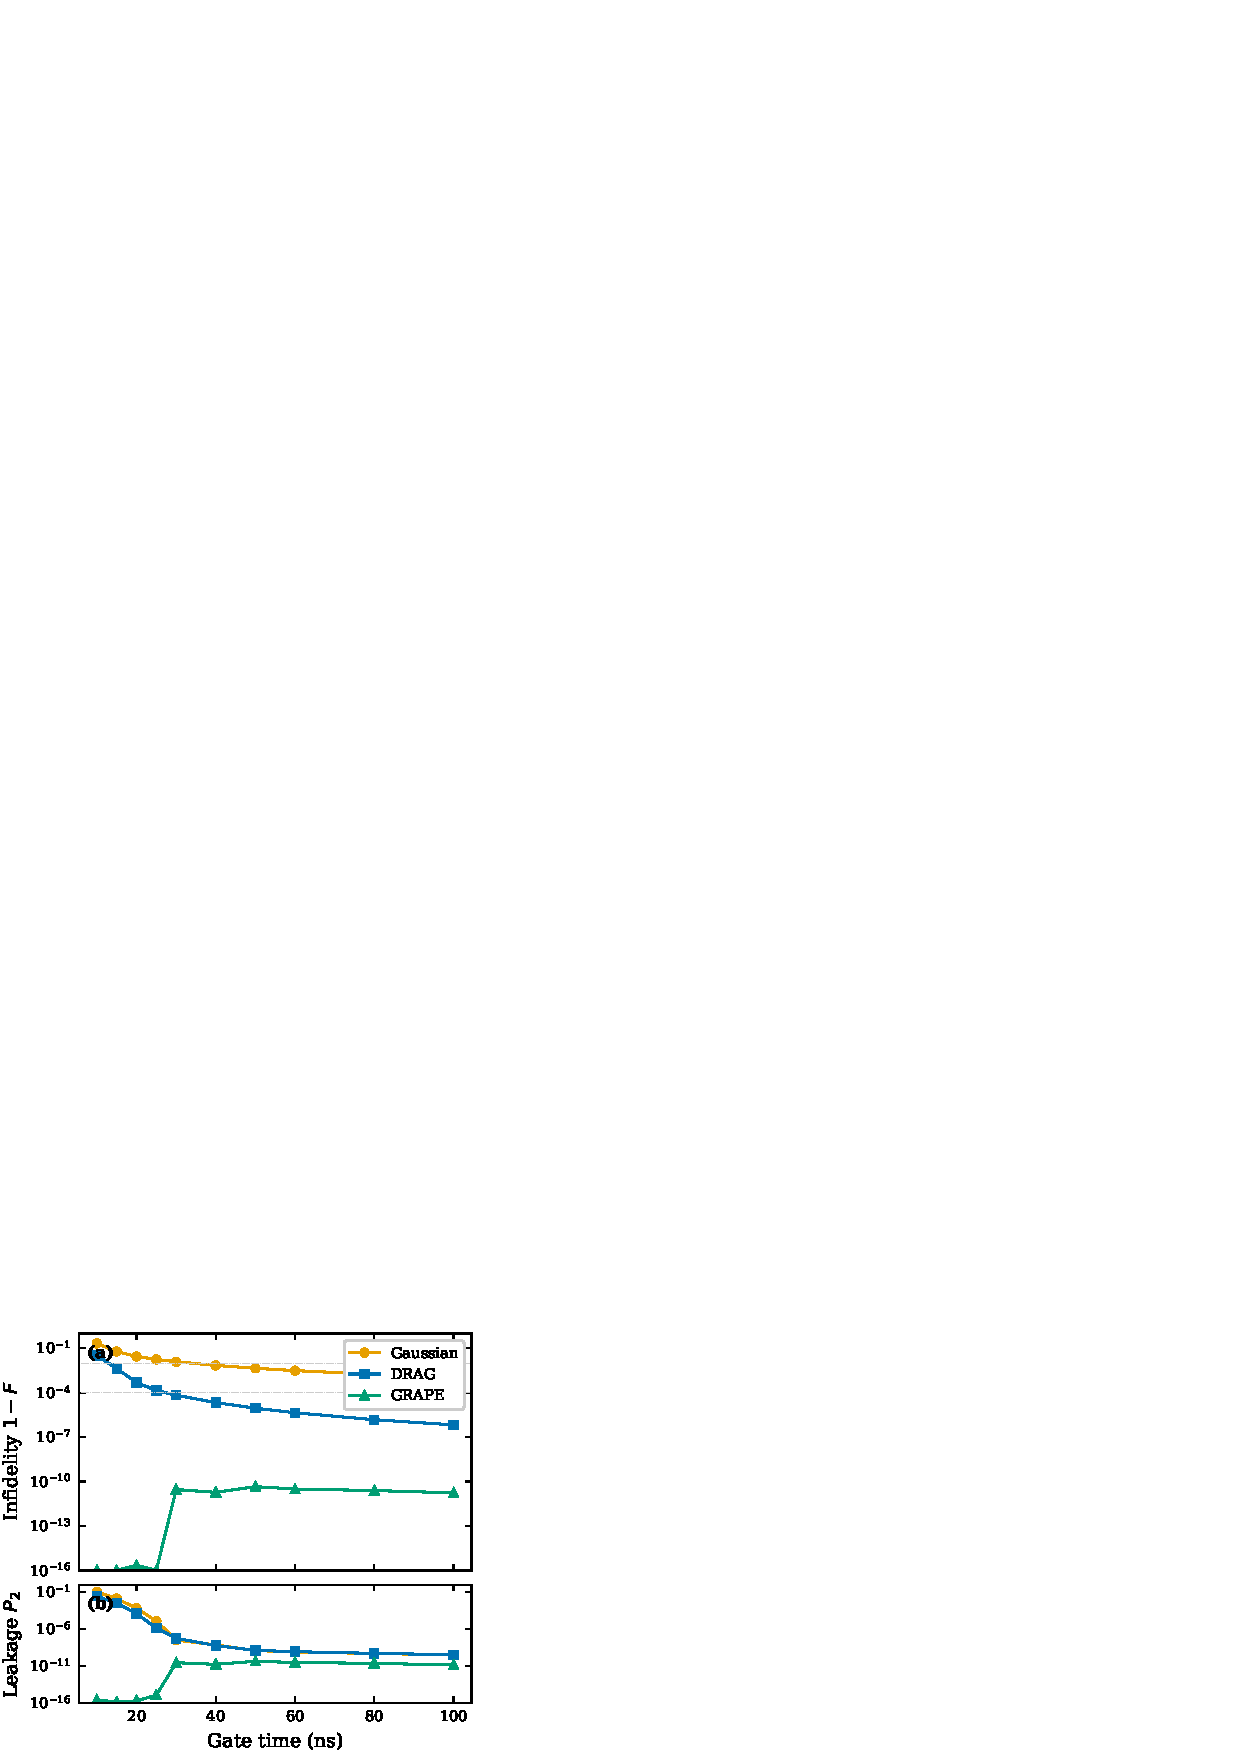
\includegraphics[width=\columnwidth]{fig2_gatetime_sweep.pdf}
\caption{Three-level X-gate performance vs.\ gate time ($\alpha/2\pi = \SI{-200}{\mega\hertz}$, closed system). (a)~Infidelity $1 - F$ on a logarithmic scale. GRAPE achieves machine-precision fidelity at all gate times. Both Gaussian and DRAG infidelities decrease monotonically. Dotted lines mark $10^{-2}$ and $10^{-4}$ infidelity levels. (b)~Leakage probability $P_2$ to the $\ket{2}$ state. DRAG's leakage suppression improves exponentially with gate time, consistent with the perturbative scaling of the first-order correction.}
\label{fig:gatetime}
\end{figure}

\subsection{Experiment C: Error budget analysis}
\label{sec:error_budget}

To decompose the error sources, we evaluate each pulse method under progressively more realistic noise models using the Lindblad master equation [Eq.~\eqref{eq:lindblad}] with IQM Garnet parameters ($T_1 = \SI{37}{\micro\second}$, $T_2 = \SI{9.6}{\micro\second}$) at a gate time of \SI{20}{\nano\second}. Table~\ref{tab:error_budget} presents the three-level error budget.

\begin{table*}[!htbp]
\caption{Error budget for the X gate at $T = \SI{20}{\nano\second}$. Infidelity $\epsilon = 1 - F$ is shown for each noise channel in both three-level and two-level models. ``Coherent'' denotes closed-system (unitary) evolution. Control noise entries show the mean infidelity over 100 random realizations. In the three-level model (upper panel), Gaussian error is dominated by coherent leakage; DRAG and GRAPE are decoherence-limited. In the two-level model (lower panel), Gaussian and GRAPE achieve identical decoherence-limited performance.}
\label{tab:error_budget}
\begin{ruledtabular}
\begin{tabular}{l ccc ccc}
& \multicolumn{3}{c}{Three-level model} & \multicolumn{3}{c}{Two-level model} \\
Error source & Gaussian $\epsilon$ & DRAG $\epsilon$ & GRAPE $\epsilon$ & Gaussian $\epsilon$ & DRAG $\epsilon$ & GRAPE $\epsilon$ \\
\hline
Coherent        & $2.8\!\times\!10^{-2}$ & $4.9\!\times\!10^{-4}$ & $<\!10^{-15}$ & $<\!10^{-8}$ & $2.8\!\times\!10^{-2}$ & 0 \\
$T_1$ only      & $2.8\!\times\!10^{-2}$ & $7.3\!\times\!10^{-4}$ & $2.1\!\times\!10^{-4}$ & $2.5\!\times\!10^{-4}$ & $2.8\!\times\!10^{-2}$ & $2.4\!\times\!10^{-4}$ \\
$T_2$ only      & $2.8\!\times\!10^{-2}$ & $6.1\!\times\!10^{-4}$ & $5.8\!\times\!10^{-4}$ & $3.8\!\times\!10^{-4}$ & $2.8\!\times\!10^{-2}$ & $3.8\!\times\!10^{-4}$ \\
$T_1 + T_2$     & $2.9\!\times\!10^{-2}$ & $8.4\!\times\!10^{-4}$ & $7.2\!\times\!10^{-4}$ & $5.8\!\times\!10^{-4}$ & $2.8\!\times\!10^{-2}$ & $5.7\!\times\!10^{-4}$ \\
Noise 1\%       & $2.8\!\times\!10^{-2}$ & $6.6\!\times\!10^{-4}$ & $2.4\!\times\!10^{-4}$ & $2.3\!\times\!10^{-4}$ & $2.8\!\times\!10^{-2}$ & $2.3\!\times\!10^{-4}$ \\
Noise 5\%       & $3.4\!\times\!10^{-2}$ & $5.6\!\times\!10^{-3}$ & $5.9\!\times\!10^{-3}$ & $5.7\!\times\!10^{-3}$ & $3.4\!\times\!10^{-2}$ & $5.7\!\times\!10^{-3}$ \\
\end{tabular}
\end{ruledtabular}
\end{table*}

The error budget (Fig.~\ref{fig:error_budget}) reveals a striking three-tier structure. For Gaussian pulses, coherent error dominates at all noise levels: adding full decoherence changes the infidelity from $2.8 \times 10^{-2}$ to $2.9 \times 10^{-2}$ (a relative change of only $\sim\!4\%$), indicating that Gaussian gate error is overwhelmingly due to leakage and rotation error, not decoherence.

For GRAPE, the coherent error vanishes to machine precision ($< 10^{-15}$), and the total error under full decoherence ($7.2 \times 10^{-4}$) represents the \emph{decoherence floor}---the minimum achievable infidelity set by the hardware's $T_1$ and $T_2$ for this gate time.

For DRAG, the picture is intermediate but remarkably close to GRAPE. The coherent infidelity of $4.9 \times 10^{-4}$ reflects the residual leakage and rotation error not captured by the first-order correction. Under full decoherence, DRAG achieves $\epsilon = 8.4 \times 10^{-4}$, only a factor of $1.2\times$ above GRAPE's decoherence floor. This is a qualitatively different regime from the Gaussian: DRAG is \emph{decoherence-limited} (the decoherence contribution $\sim\!3.5 \times 10^{-4}$ is comparable to the coherent contribution $4.9 \times 10^{-4}$), whereas the Gaussian is entirely \emph{coherent-error-limited}.

The decoherence floor can be estimated analytically. For a gate of duration $T$ with relaxation rate $\gamma_1 = 1/T_1$ and dephasing rate $\gamma_\phi = 1/T_2 - 1/(2T_1)$, the leading-order infidelity contributions are~\cite{wood2018quantification}
\begin{equation}
\epsilon_{T_1} \approx \frac{T}{2T_1}, \quad \epsilon_\phi \approx \frac{T}{T_2} - \frac{T}{2T_1}.
\label{eq:decoherence_floor}
\end{equation}
For $T = \SI{20}{\nano\second}$, $T_1 = \SI{37}{\micro\second}$, $T_2 = \SI{9.6}{\micro\second}$, this gives $\epsilon_{T_1} \approx 2.7 \times 10^{-4}$ and $\epsilon_\phi \approx 1.8 \times 10^{-3}$, consistent with GRAPE's measured $T_1$-only infidelity of $2.1 \times 10^{-4}$ and $T_2$-only infidelity of $5.8 \times 10^{-4}$.

At $5\%$ control noise, both DRAG and GRAPE degrade significantly ($5.6 \times 10^{-3}$ and $5.9 \times 10^{-3}$, respectively), with DRAG actually performing slightly \emph{better} than GRAPE. This suggests that DRAG's simpler pulse shape may provide marginally better resilience to large amplitude perturbations.


\begin{figure}[!htbp]
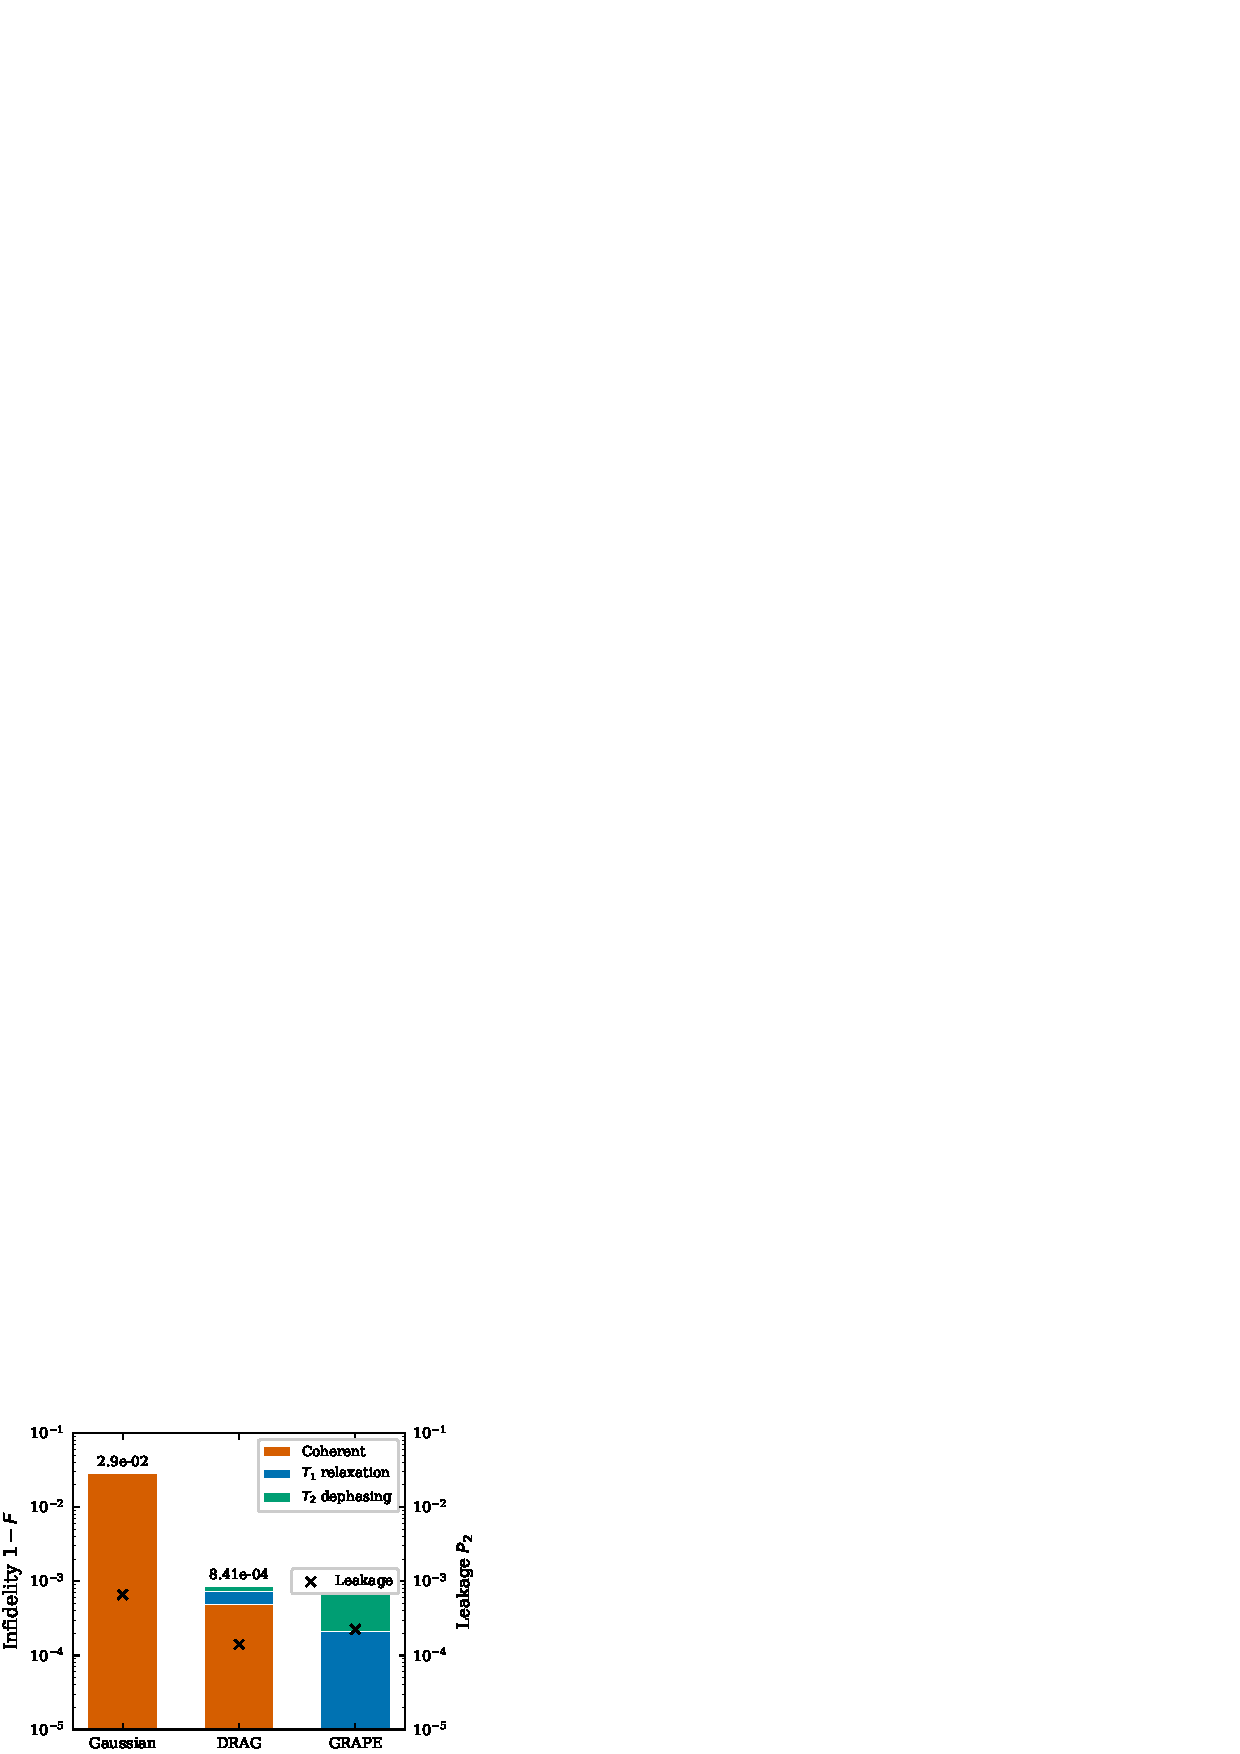
\includegraphics[width=\columnwidth]{fig4_error_budget.pdf}
\caption{Error budget decomposition for the X gate in the three-level transmon model at $T = \SI{20}{\nano\second}$ with IQM Garnet parameters. Stacked bars show the contributions of coherent error (red), $T_1$ relaxation (blue), and $T_2$ dephasing (green) to the total infidelity. Numerical values above each bar indicate the total infidelity under full decoherence. Black crosses show the leakage probability $P_2$ (right axis). Gaussian error is dominated by coherent leakage; DRAG and GRAPE are decoherence-limited. GRAPE's zero coherent error is not visible at this scale.}
\label{fig:error_budget}
\end{figure}

The two-level error budget (right columns of Table~\ref{tab:error_budget}) confirms that GRAPE's advantage in the three-level model arises entirely from leakage suppression, not from a superior two-level rotation. In two levels (no leakage), Gaussian and GRAPE perform identically---both are decoherence-limited ($\epsilon \approx 5.8 \times 10^{-4}$). DRAG in two levels shows coherent infidelity of $2.8 \times 10^{-2}$, dominated by the parasitic quadrature rotation that serves no purpose without a $\ket{2}$ state.

\subsection{Experiment D: Robustness analysis}
\label{sec:robustness}

We evaluate robustness by sweeping two common calibration errors: (i) qubit frequency detuning $\delta\omega/2\pi \in [-5, +5]$ MHz, implemented as an additional term $\delta\omega \cdot \hat{n}$ in the Hamiltonian, and (ii) systematic amplitude error $\epsilon_a \in [-5\%, +5\%]$, implemented by scaling all pulse amplitudes by $(1 + \epsilon_a)$. Each sweep uses 41 linearly spaced points.

Table~\ref{tab:robustness} summarizes the results for the three-level model.

\begin{table}[!htbp]
\caption{Robustness of X-gate fidelity in the three-level model under detuning ($\delta\omega/2\pi \in \pm\SI{5}{\mega\hertz}$) and amplitude error ($\epsilon_a \in \pm 5\%$). ``Nom.'' is the nominal (zero-error) fidelity; ``Min'' and ``Mean'' are over the sweep range.}
\label{tab:robustness}
\begin{ruledtabular}
\begin{tabular}{l ccc ccc}
& \multicolumn{3}{c}{Detuning} & \multicolumn{3}{c}{Amplitude} \\
Method & Nom. & Min & Mean & Nom. & Min & Mean \\
\hline
Gaussian & 0.972 & 0.937 & 0.969 & 0.972 & 0.965 & 0.970 \\
DRAG     & 0.999 & 0.990 & 0.997 & 0.999 & 0.990 & 0.997 \\
GRAPE    & 1.000 & 0.931 & 0.976 & 1.000 & 0.994 & 0.998 \\
\end{tabular}
\end{ruledtabular}
\end{table}

The robustness results (Fig.~\ref{fig:robustness}) reveal a nuanced picture. GRAPE shows excellent amplitude robustness: even at $\pm 5\%$ amplitude error, the minimum fidelity remains 0.994, the best among all three methods. DRAG also shows strong amplitude robustness (minimum 0.990), significantly outperforming Gaussian (minimum 0.965).

For detuning, DRAG is the \emph{most robust} method, with a minimum fidelity of 0.990 over $\pm\SI{5}{\mega\hertz}$ detuning, compared to 0.937 for Gaussian and 0.931 for GRAPE. GRAPE's minimum detuning fidelity is actually the \emph{lowest} of all three methods. This arises because GRAPE-optimized pulse shapes contain richer spectral content that can couple more strongly to off-resonant transitions when the qubit frequency shifts. In contrast, DRAG's smooth analytical pulse shape and frequency-independent $\beta$ provide natural resilience to small frequency offsets. This finding is consistent with the known sensitivity of numerically optimized pulses to parameter variations~\cite{propson2022robust} and motivates incorporating detuning robustness directly into the GRAPE cost function~\cite{wilhelm2020introduction, goerz2014optimal}.


\begin{figure*}[!htbp]
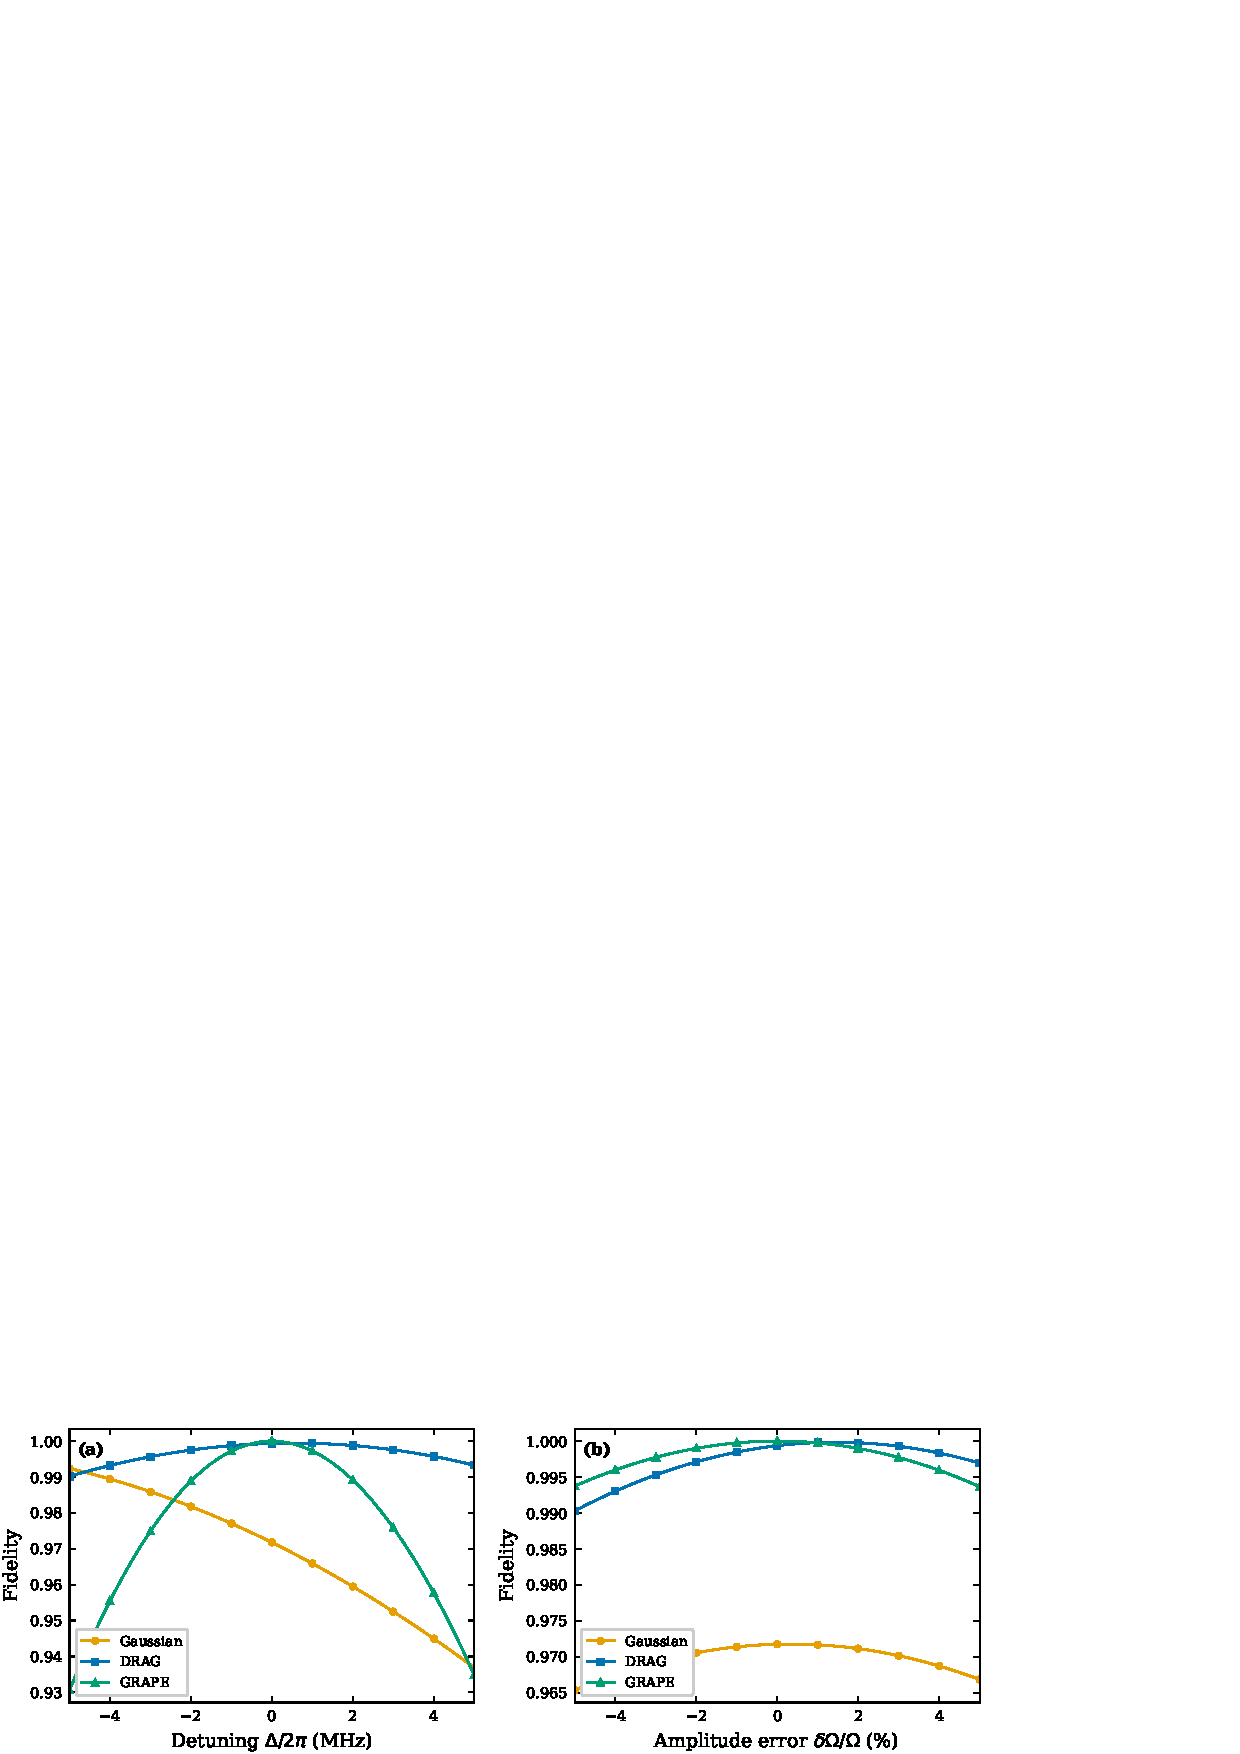
\includegraphics[width=\textwidth]{fig3_robustness.pdf}
\caption{Robustness of X-gate fidelity in the three-level transmon model ($T = \SI{20}{\nano\second}$, $\alpha/2\pi = \SI{-200}{\mega\hertz}$, closed system). (a)~Fidelity vs.\ qubit frequency detuning over $\pm\SI{5}{\mega\hertz}$. DRAG (blue) maintains the highest minimum fidelity (0.990), outperforming both Gaussian (orange, 0.937) and GRAPE (green, 0.931). GRAPE's sensitivity arises from its richer spectral content coupling to off-resonant transitions. (b)~Fidelity vs.\ systematic amplitude error over $\pm 5\%$. GRAPE shows the best amplitude robustness (minimum 0.994), followed by DRAG (0.990) and Gaussian (0.965).}
\label{fig:robustness}
\end{figure*}

%==============================================================================
\section{Discussion}
\label{sec:discussion}
%==============================================================================

\subsection{The three-level model as the appropriate comparison arena}

Our results clearly demonstrate that the two-level model is inadequate for comparing GRAPE to analytical pulse methods. In two levels, a properly calibrated Gaussian pulse achieves near-unit fidelity (Table~\ref{tab:2level}), and there is nothing for GRAPE to improve upon---both methods hit the decoherence floor. The three-level model introduces leakage as a physically relevant error source that analytical corrections (DRAG) partially suppress and that GRAPE can fully eliminate.

This finding has implications for how GRAPE results are reported in the literature. Claims of large fidelity improvements based on two-level comparisons against uncalibrated baselines may overstate GRAPE's practical advantage. The meaningful comparison is in the multi-level model with a properly calibrated analytical baseline.

\subsection{The importance of correct DRAG calibration}

A key finding of this work is the critical importance of correctly implementing the DRAG parameter $\beta$. The formula $\beta = -1/(2\alpha)$~\cite{motzoi2009simple} yields an amplitude-independent, $O(1)$ quantity ($\beta = 0.398$ for $\alpha/2\pi = \SI{-200}{\mega\hertz}$) that provides effective first-order leakage suppression across all gate times tested. This is in sharp contrast to alternative formulas appearing in the literature that express $\beta$ as a function of the peak Rabi frequency $\Omega_\text{max}$, which would yield amplitude-dependent values and incorrect gate-time scaling.

With the correct $\beta$, DRAG fidelity improves monotonically with gate time (Table~\ref{tab:3level}), precisely as expected from perturbation theory: as the gate time increases and $\Omega_\text{max}$ decreases, the ratio $\Omega/|\alpha|$ shrinks and higher-order corrections become negligible. At \SI{100}{\nano\second}, DRAG achieves $F > 0.999999$, indistinguishable from unity at the precision of typical experiments.

In experimental practice, $\beta$ is typically calibrated empirically using AllXY or similar sequences~\cite{chen2016measuring, sheldon2016procedure}. Our results confirm that such calibration is essential and that the analytical formula serves as an accurate starting point when unit consistency is maintained.

\subsection{Error hierarchy and the decoherence floor}

The error budget (Table~\ref{tab:error_budget}) reveals a clear hierarchy for the three-level model at \SI{20}{\nano\second}:

\begin{enumerate}
\item \emph{Coherent error} (leakage + rotation error): Dominates for Gaussian ($\epsilon = 2.8 \times 10^{-2}$). Significantly suppressed by DRAG ($\epsilon = 4.9 \times 10^{-4}$). Eliminated by GRAPE ($\epsilon < 10^{-15}$).

\item \emph{Dephasing} ($T_2$): For GRAPE, contributes $5.8 \times 10^{-4}$ to infidelity. This is the dominant decoherence channel given $T_2 = \SI{9.6}{\micro\second} \ll 2T_1 = \SI{74}{\micro\second}$.

\item \emph{Relaxation} ($T_1$): Contributes $2.1 \times 10^{-4}$, smaller than dephasing due to the longer $T_1$.

\item \emph{Control noise} ($\sigma = 1\%$): For GRAPE, contributes $2.4 \times 10^{-4}$, comparable to $T_1$. At $\sigma = 5\%$, control noise ($5.9 \times 10^{-3}$) exceeds the decoherence floor and becomes the dominant error source for both DRAG and GRAPE.
\end{enumerate}

The central quantitative finding is that GRAPE outperforms Gaussian by $39\times$ in the three-level model with full decoherence, but outperforms DRAG by only $1.2\times$. This modest advantage arises because properly calibrated DRAG already suppresses coherent leakage error to the point where decoherence dominates. GRAPE's advantage over DRAG is primarily qualitative: it guarantees \emph{zero} coherent error to machine precision, providing a safety margin that first-order perturbative corrections cannot match. This distinction becomes practically significant at shorter gate times (Table~\ref{tab:3level}) or for higher-precision applications approaching the fault-tolerance threshold.

This hierarchy suggests that for IQM Garnet--class hardware, improving $T_2$ (through better materials, filtering, or dynamical decoupling) would have the greatest impact on achievable gate fidelity, while control noise at the $\sim 1\%$ level is already subdominant.

\subsection{Robustness tradeoffs}

The robustness analysis (Table~\ref{tab:robustness}) reveals an important practical consideration: DRAG's detuning robustness (minimum fidelity 0.990) exceeds both Gaussian (0.937) and GRAPE (0.931). This arises from two factors. First, DRAG's smooth, analytically determined pulse shape avoids the sharp spectral features that make GRAPE pulses sensitive to frequency offsets. Second, the DRAG correction $\beta = -1/(2\alpha)$ is independent of the qubit frequency, so moderate detuning does not invalidate the correction (though it does shift the effective anharmonicity seen by the pulse).

For amplitude errors, GRAPE retains a slight advantage (minimum 0.994 vs.\ 0.990 for DRAG), likely because the numerical optimizer finds a broad fidelity maximum in the amplitude landscape. Both methods significantly outperform uncorrected Gaussian pulses (minimum 0.965).

These findings suggest that the choice between DRAG and GRAPE in practice depends on the dominant calibration uncertainty. For systems where frequency drift is the primary concern (e.g., charge-noise-limited transmons), DRAG may actually be \emph{preferable} to unconstrained GRAPE. For systems where amplitude calibration is the bottleneck, GRAPE offers a modest but consistent advantage. Robust optimal control methods~\cite{propson2022robust, goerz2014optimal} that incorporate parameter uncertainty into the GRAPE cost function could potentially achieve the best of both approaches.

\subsection{Limitations}

Several limitations of this work should be acknowledged:

\begin{itemize}
\item \textit{Simulation only.} All results are from numerical simulation. No pulses were executed on physical hardware. The framework demonstrates API connectivity to IQM Garnet and retrieves system topology, but hardware validation remains future work.

\item \textit{Closed-system GRAPE.} The GRAPE optimization uses closed-system (unitary) fidelity as the cost function. Open-system GRAPE~\cite{schulte2011optimal} incorporating Lindblad dynamics during optimization could potentially discover pulses that partially compensate for decoherence, further improving performance.

\item \textit{Markovian noise.} The Lindblad model assumes Markovian dynamics. Low-frequency $1/f$ noise and non-Markovian effects~\cite{norris2016qubit}, which are significant in superconducting qubits, are not captured.

\item \textit{Single-qubit gates only.} Extension to two-qubit gates (CZ, CNOT) is computationally more demanding and involves additional physics (e.g., parasitic ZZ coupling).

\item \textit{Static parameters.} We use fixed calibration parameters; real hardware exhibits temporal drift in $\omega_q$, $T_1$, and $T_2$.

\item \textit{Analytical DRAG only.} We use the analytical $\beta$ formula rather than numerical optimization of $\beta$. Numerically optimized DRAG~\cite{theis2018counteracting, motzoi2013backaction} could further improve performance, though it would still be limited to the functional form of Eq.~\eqref{eq:drag}.
\end{itemize}

%==============================================================================
\section{Conclusion}
\label{sec:conclusion}
%==============================================================================

We have presented a systematic comparison of Gaussian, DRAG, and GRAPE control pulses for single-qubit gates in a three-level transmon model with hardware-representative parameters. The principal findings are:

(1) GRAPE achieves unit closed-system fidelity ($1 - F < 10^{-15}$) with negligible leakage ($P_2 < 10^{-15}$) across all tested gate times (10--\SI{100}{\nano\second}), while Gaussian pulses retain significant coherent errors dominated by leakage.

(2) Properly calibrated DRAG (with $\beta = -1/(2\alpha) = 0.398$) provides excellent first-order leakage suppression, achieving $F = 0.9995$ at \SI{20}{\nano\second} and $F > 0.999999$ at \SI{100}{\nano\second}. DRAG fidelity improves monotonically with gate time, confirming the effectiveness of the analytical correction when the DRAG parameter is correctly computed as an amplitude-independent quantity.

(3) Under realistic decoherence ($T_1 = \SI{37}{\micro\second}$, $T_2 = \SI{9.6}{\micro\second}$), GRAPE reaches the decoherence floor ($\epsilon = 7.2 \times 10^{-4}$), outperforming Gaussian by $39\times$. DRAG achieves $\epsilon = 8.4 \times 10^{-4}$, only $1.2\times$ above GRAPE, indicating that DRAG is already near the decoherence floor at this gate time. GRAPE's primary advantage is the complete elimination of coherent error.

(4) DRAG exhibits superior detuning robustness compared to both Gaussian and GRAPE (minimum fidelity 0.990 vs.\ 0.931 for GRAPE over $\pm\SI{5}{\mega\hertz}$). GRAPE retains the best amplitude robustness (minimum 0.994). The choice between DRAG and GRAPE in practice should account for the dominant source of calibration uncertainty.

These results quantify the regime where numerical optimal control provides a genuine advantage over analytical pulse methods: short gate times ($T \lesssim \SI{15}{\nano\second}$) where higher-order leakage pathways dominate, and applications requiring guaranteed zero coherent error. For longer gate times with moderate detuning uncertainty, properly calibrated DRAG may offer comparable or superior performance to unconstrained GRAPE. Future work will extend to open-system GRAPE optimization, two-qubit entangling gates, robust cost functions incorporating parameter uncertainty~\cite{propson2022robust, goerz2014optimal}, and hardware validation on physical transmon processors.

\begin{acknowledgments}
The author thanks Embry-Riddle Aeronautical University for research support. The QubitPulseOpt framework is open source and available at \url{https://github.com/rylanmalarchick/QubitPulseOpt}.
\end{acknowledgments}

\appendix

\section{AI Disclosure}
AI-assisted tools (Claude, Anthropic) were used for code development, debugging, and manuscript preparation. All scientific concepts, experimental design, analysis, and interpretation were performed by the author. The author takes full intellectual responsibility for all content.

\bibliography{references}

\end{document}
